\chapter{Hardware}\label{ch:hardware}

The hardware modules used for this project are described in this chapter. The connection of these system parts is described in chapter \ref{ch:system}. The hardware was provided by the university.

\section{Cohda Wireless}

Cohda Wireless develops different soft- and hardware for intelligent transport systems (ITS). Their product range reaches from modules for autonomous vehicles in mining operations to connected autonomous vehicle (CAV) systems \cite{cohda_wireless}. One of these products is the MK5, which is an interface between the board computer in the car and other V2X users. For this thesis, the MK5 is used to establish a wireless connection between a vehicle and a charging station.

The MK5 has two major functional components. The u-blox THEO-P1 module for the wireless communication and a processor subsystem for the application. The application processor runs a Linux operation system and application software for intelligent transport systems. The operation system is an embedded Linux based on Ubuntu 14.04 LTS. Figure \ref{fig:MK5_Stack} shows the software block diagram of the MK5. In this thesis, only the European standard is used. 

\begin{figure}[htb]
	\centering
	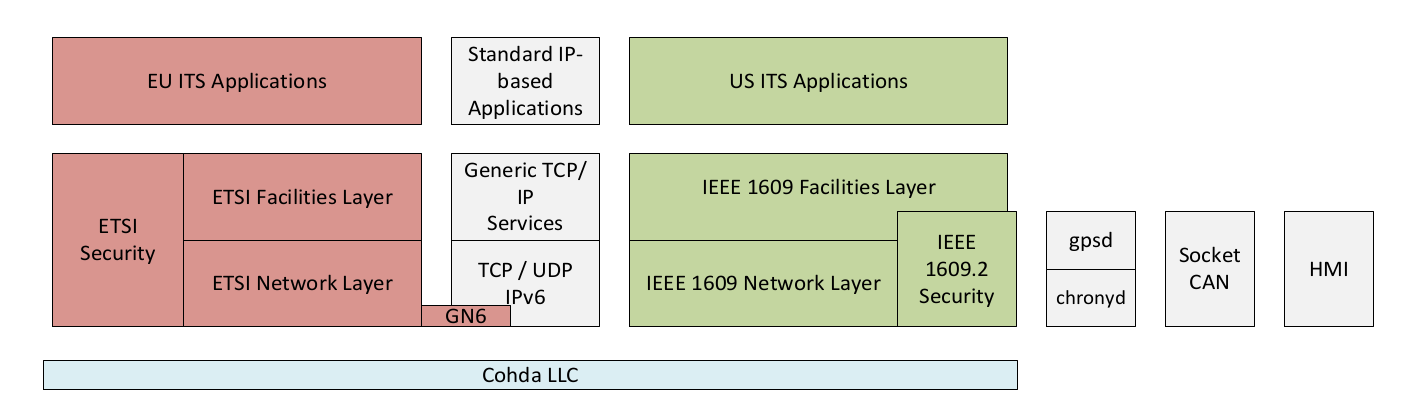
\includegraphics[width=1\textwidth]{images/MK5_Stack.png}
	\caption{MK5 Software Block Diagram \cite{MK5_Datasheet}}
	\label{fig:MK5_Stack}
\end{figure}

\newpage

\subsection{Cohda Wireless DSRC Radio}

The mobility radio contains two components. The Media Access Control (MAC) and the Physical Layer (PHY).

\subsubsection{Cohda Wireless PHY}

The Cohda Wireless PHY is an IEEE 802.11p compliant physical layer radio transceiver with two independent PHY modules for single or dual radio DSRC systems. Following operating modes and functionalities are supported:
\begin{itemize}
	\item Single-channel mode (1 or 2 antenna diversity operation)
	\item Dual-channel mode (1 antenna per channel), 2 independent IEEE 802.11p radios operating on different radio channels.
	\item 10\;MHz (DSRC) channel bandwidth modes.
	\item Dual 5.x\;GHz RF paths (5.18\;GHz to 5.93\;GHz).
	\item Transmit mask meeting IEEE 802.11p Class C (5\;GHz band).
	\item IEEE 802.11p enhanced adjacent channel receiver performance.
	\item Transmit antenna cyclic delay diversity (2 antenna operation only).
	\item Transmit power control (0.5\;dB steps).
	\item Fast mode changes for synchronized channel switching systems.
\end{itemize}

\subsubsection{Cohda Wireless MAC}

The Cohda Wireless MAC implements a full IEEE 802.11p compliant MAC layer which provides a fast and time-synchronized channel switching functionality. \cite{MK5_Datasheet}

\newpage

\subsection{Onboard Unit}

The Onboard Unit (OBU) has three antenna connectors. One is used for GNSS and the other two for 802.11p. There is also an SD card slot for saving log data. On the other side of the housing there is a power, a USB and a D-SUB DE-9 connector. The latter is intended for a CAN bus interface to the board computer. The Ethernet port is used to program the OBU with a computer or to transmit data, which can be sent wireless to other hosts. Inside the OBU there is an MK5 Board with an NXP chip on it, which runs a Cohda Wireless firmware. \cite{Cohda_Wireless_Hardware}

\begin{figure}[htb]
	\centering
	\begin{minipage}{.5\textwidth}
		\centering
		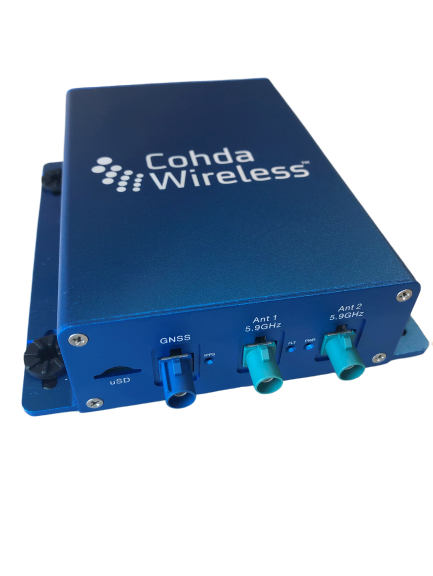
\includegraphics[width=0.4\linewidth]{images/OBUantenna}
		\caption{OBU Antenna Side}
		\label{fig:OBUantenna}
	\end{minipage}%
	\begin{minipage}{.5\textwidth}
		\centering
		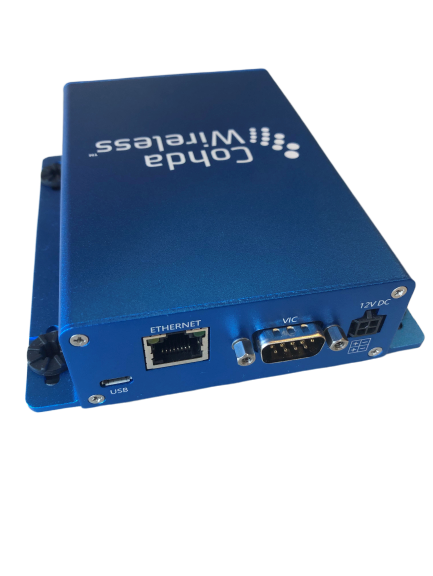
\includegraphics[width=0.4\linewidth]{images/OBUpower}
		\caption{OBU Power and Data Side}
		\label{fig:OBUpower}
	\end{minipage}
\end{figure}

\subsection{Roadside Unit}

The Roadside Unit (RSU) contains the same MK5 carrier board as the OBU, but has only antenna sockets and an Ethernet port. The housing around the module is built to protect the board inside from water. Additionally there is a Power over Ethernet extractor inside to separate the power, which comes from the Ethernet port, so that the whole RSU can be supplied with power. \cite{MK5_Datasheet} \cite{Cohda_Wireless_Hardware}

\begin{figure}[htb]
	\centering
	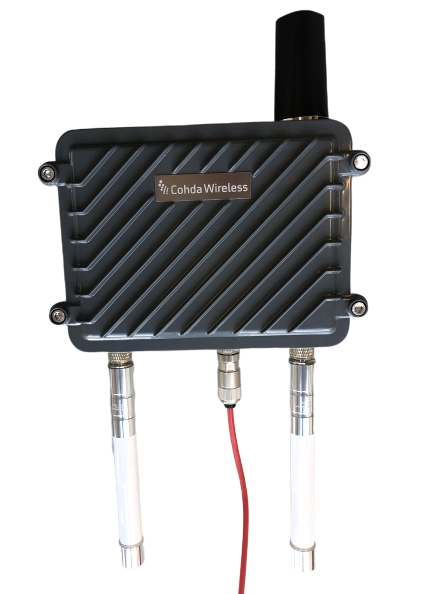
\includegraphics [width=0.3\textwidth] {images/RSU}
	\caption{RSU in waterproof Housing}
	\label{fig:RSU}
\end{figure}

%--------------------------------------------------------------------------------------------------

\section{Charging Device}\label{sec:chargingDevices}

For this project, there are two different charging devices. Both are produced by KEBA and are called P30. They can provide up to 22\;kW of charging power. Both can be unlocked with a RFID card. These devices are designed for integration into a smart grid application, where the vehicle only charges, if there is enough power in the system. Therefore the device is not tailored for this project.

One of the devices is called b-series and can be unlocked with a single relay switch. It is not possible to lock its charging port once it is released, until the vehicle is unplugged. A potential-free contact inside the device shows if the vehicle is plugged in or not. 

The other type is called c-series. Its main difference is the interface to the system. It communicates over an Ethernet port with its control unit. The communication happens over UDP. The advantage of this version is, that the control unit knows the state of the charging device. The states are called  \textit{startup, not ready, ready for charging, charging, error and charging interrupted}. Additional parameters, for example the maximum charging current or an energy limit for a charging session, can be set. This version has an additional display on the front. It shows messages, which are received over Ethernet.
\cite{KEBAP30_Datasheet} \cite{KEBAP30_Comparisonsheet} \cite{KEBAP30_UDP_Programmers_Guide}


\begin{figure}[htb]
	\centering
	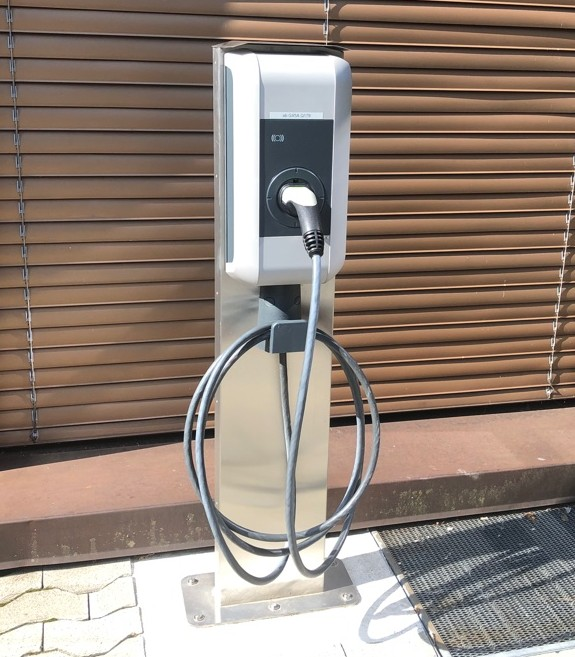
\includegraphics [width=0.6\textwidth] {images/ChargingStationB}
	\caption{KEBA P30 Charging Station installed on HSR campus}
	\label{fig:ChargingStation}
\end{figure}

\section{ICOM Wireless Research Vehicle}

The institute ICOM at HSR has an electric vehicle, which can be used to run some measurements in real environments outside and in movement. It is a rebuilt Opel Ampera. The vehicle is equipped with the following tools: \cite{ICOMWirelessResearchVehicle}

\begin{itemize}
	\item Onboard power supply (1\;kW)
	\item Constant internet connection with 4G/LTE
	\item High-performance computer for calculations
	\item GNSS localization and synchronized Rubidium time base
	\item Plenty of room for more 19" rack measure equipment
    \item A roof box for antennas and more devices
\end{itemize}

\begin{figure}[htb]
	\centering
	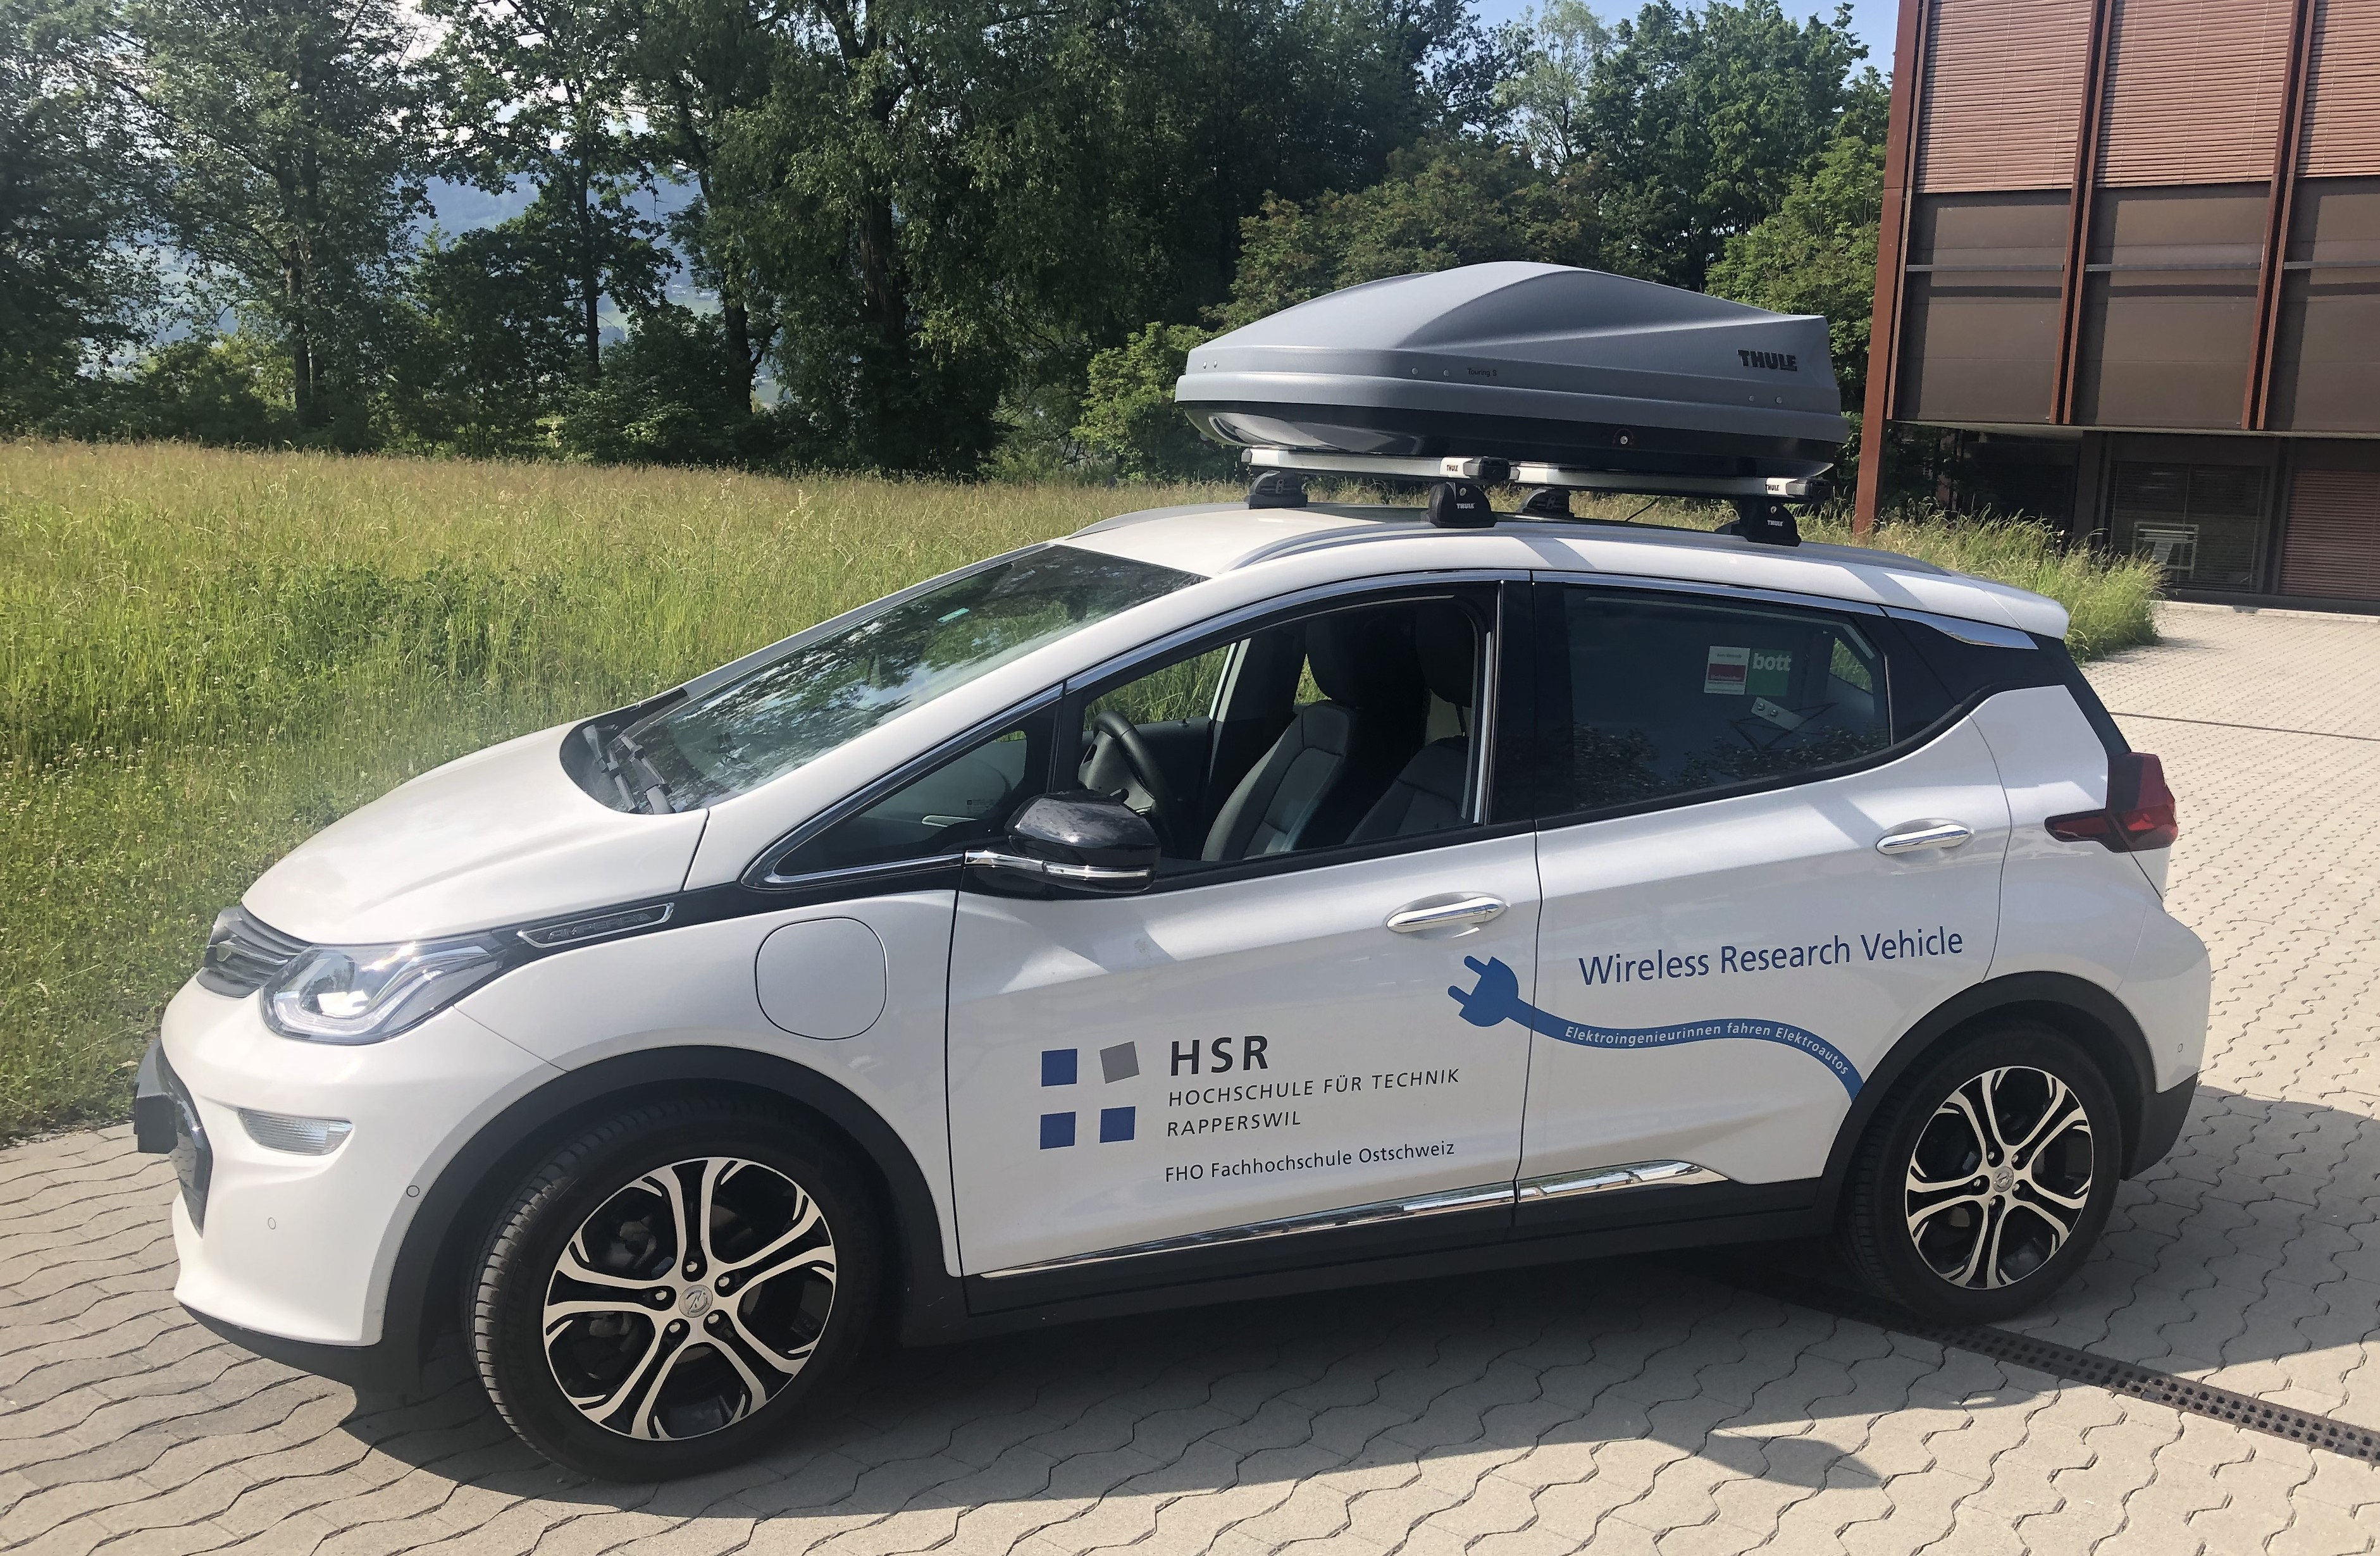
\includegraphics [width=0.8\textwidth] {images/WRV}
	\caption{ICOM Wireless Research Vehicle}
	\label{fig:WRV}
\end{figure}

\newpage

\section{Raspberry Pi}

The Raspberry Pi is a small single-board computer which runs Linux. It is very cheap compared to a normal desktop computer. Additionally it has some in- and outputs, which can be controlled by the software on it. In this project, the two Raspberry Pis are used to control the whole system and one as a stream server as described in chapter \ref{ch:system}.

\begin{figure}[htb]
	\centering
	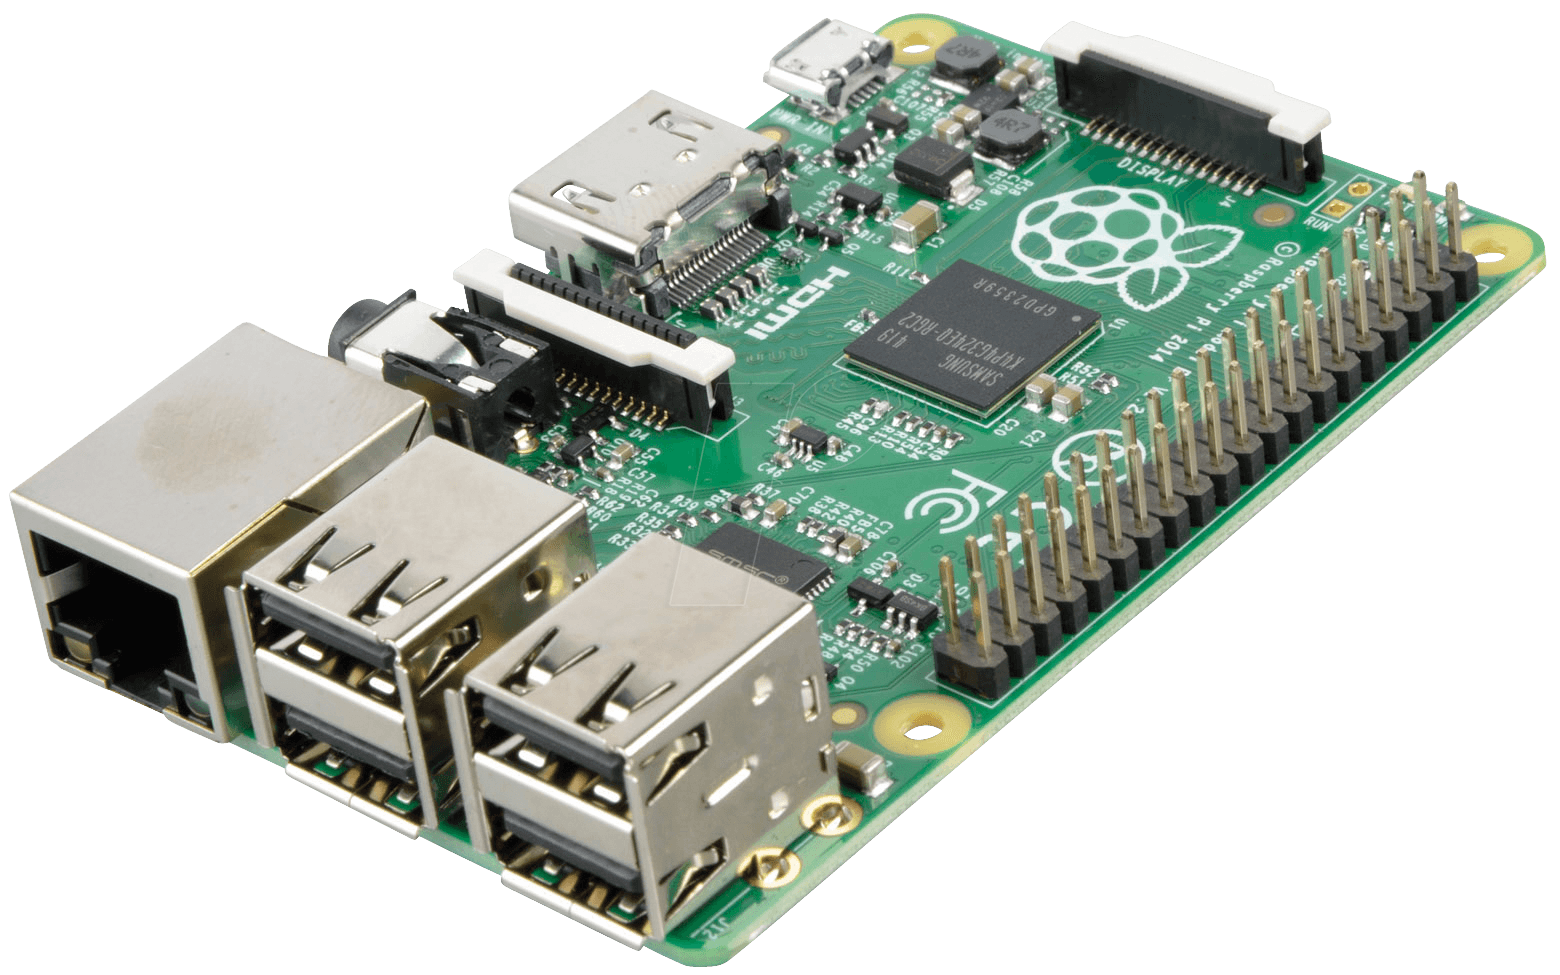
\includegraphics [width=0.4\textwidth] {images/RPi}
	\caption{Raspberry Pi \cite{RaspberryPi}}
	\label{fig:RPi}
\end{figure}

\section{SparkFun GPS-RTK2 Board ZED-F9P}

SparkFun offers a board with an u-blox ZED-F9P module on it. The module is able to receive GPS, GLONASS, Galileo and BeiDou simultaneously. It has a high refresh rate to get multiple measurements per second. With this board, it is easy to configure the u-blox module over u-center. So it can be used for RTK applications, as required in this project. Depending on the configuration of the module, it is set as a base station, which knows its position and generates correction data. It sends the data to a movable GNSS module, called a rover. Moreover, the module can be configured as a rover, to receive the data and calculate the exact position.
\cite{ZED-F9P-Modul}
\cite{ZED-F9P-IntegrationManual}

\begin{figure}[htb]
	\centering
	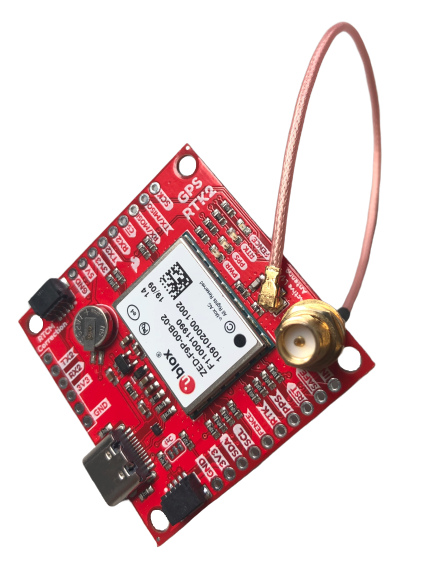
\includegraphics[angle=270, width=0.5\textwidth]{images/ZED-F9P}
	\caption{SparkFun GPS-RTK2 Board ZED-F9P}
	\label{fig:ZED F9P}
\end{figure}


